\section{Approximation by Orthogonal Indicator Tiles}\label{sec:part4}

\begin{enumerate}[(a)]
\item A sample of tiles on $I$, where tiles with different colors correspond to $E_a, E_b, E_c$.

\begin{center}
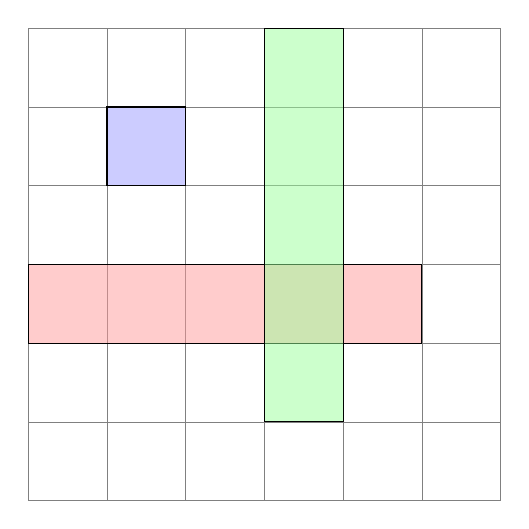
\begin{tikzpicture}
\draw[step=1cm,gray,very thin] (0,0) grid (6,6);
\fill[red!40!white, draw=black, fill opacity=0.5] (0,2) rectangle (5,3);
\fill[green!40!white, draw=black, fill opacity=0.5] (3,6) rectangle (4,1);
\fill[blue!40!white, draw=black, fill opacity=0.5] (1,4) rectangle (2,5);
\end{tikzpicture}
\end{center}

\item Since $\dim(\text{span}\{\phi_a\}_{a \in A}) \leq \abs{A} < \abs{I} = \dim(\mathbb{R}^I)$,  $\{\phi_a\}_{a \in A}$ cannot span $I$. Hence, it is not a basis or a frame.

\item For $u,v \in A$ s.t. $u \neq v$. If $\phi_u \perp \phi_v$
\[\innerprod{\phi_{u}}{phi_{v}} = \sum_{i \in I} \phi_{u}[i] \phi_ {v}[i] = \abs{E_u \bigcap E_v} = \lambda\delta_{u,v} = \begin{cases}
1, & u=v\\
0, & \text{else}
\end{cases} = 0 \qquad(u \neq v)\]
It means that $E_u \bigcap E_v = \emptyset$. For example, in the sample figure in part (a), the blue tile is orthogonal with the red and the green tiles, but the red and green are not orthogonal.

\item Since $\{\phi_a\}_{a \in A}$ are orthogonal, the best approximation of $x$ is its projection on the space spanned by normalized $\{\phi_a\}_{a \in A}$, i.e.
\[\hat{x} = \sum_{a \in A} \frac{\innerprod{x}{\phi_a}}{\norm{\Phi_a}^2} \phi_a.\]

\item If $\{\phi_a\}_{a \in A}$ are not orthogonal, we can construct the corresponding set orthogonal bases using Gram-Schmidt algorithm and project $x$ on it.

\end{enumerate}